\documentclass[journal,draftclsnofoot,10pt,onecolumn]{IEEEtran}
\usepackage[T1]{fontenc}
\usepackage[utf8]{inputenc}
\usepackage{amsmath,amssymb,amsfonts}
\usepackage{graphicx}
\usepackage{booktabs}
\usepackage{multirow}
\usepackage{array}
\usepackage{cite}
\usepackage{url}
\usepackage{xcolor}
\usepackage{algorithm}
\usepackage{algorithmic}
\usepackage{balance}
\graphicspath{{./}}

\begin{document}

\title{FMBM-Net: A Federated Multi-Scale Bio-Multimodal Network\\
with Latent Cross-Attention Transformer for\\
Privacy-Preserving Biomedical AI}

\author{Subrahmanyam~Tanala,~\IEEEmembership{Member,~IEEE}%
\thanks{S.~Tanala is with the Department of Electrical and Electronics
Engineering, Anil Neerukonda Institute of Technology and Sciences (ANITS),
Visakhapatnam 531162, India (e-mail: tanala.subrahmanyam@anits.edu.in).}%
\thanks{Manuscript received May 2026. Supported in part by ANITS Seed
Research Grant No.~ANITS/SRG/2025-26/EEE-04. Code, pre-processed splits,
and training scripts are available at
\texttt{https://github.com/subrahmanyamtanala-rgb/fmbm-net} (anonymous review link:
\texttt{https://anonymous.4open.science/r/fmbm-net-review}).}}

% Running headers removed for submission per IEEE author guidelines

\maketitle
% \IEEEpeerreviewmaketitle  % Uncomment for double-blind peer review

\begin{abstract}
We propose the \textbf{Federated Multi-Scale Bio-Multimodal Network
(FMBM-Net)}, a novel architecture for privacy-preserving integration of
genomic sequences, three-dimensional volumetric medical images, and
electronic health records~(EHR). The core contribution is the
\textbf{Federated Latent Cross-Attention Transformer~(FLCAT)}, which
performs $H$-head cross-modal attention with complete residual connections
and layer normalization entirely within a $(\varepsilon,\delta)$-differentially
private latent space. FMBM-Net further incorporates a boundary-guided
\textbf{Region Uncertainty Estimation~(RUE)} module and a deterministic
\textbf{Risk-Stratified Governance Controller~(RSGC)} \emph{designed to
align with} emerging healthcare AI regulatory frameworks. We evaluate
FMBM-Net on four real public benchmarks---CADD~v1.7 ($n\!=\!35{,}000$),
MSD Pancreas-CT ($n\!=\!281$ volumes), MIMIC-IV~v2.2 ($n\!=\!52{,}143$),
and a curated TCGA-LUNG multimodal cohort ($n\!=\!1{,}000$)---using
\textbf{10 independent seeds} and \textbf{bootstrap 95\,\% confidence
intervals}. FMBM-Net achieves multimodal AUROC $0.947{\pm}0.007$,
CT Dice $0.934{\pm}0.011$, GradCAM++ IoU $0.634{\pm}0.029$, and
expert-agreement score~$0.76{\pm}0.03$ at $\varepsilon\!=\!2.0$,
$\delta\!=\!10^{-5}$. All improvements over MOON are statistically
significant (Wilcoxon signed-rank, $p\!<\!0.01$; Cohen's $d\!\geq\!1.2$).
\end{abstract}

\begin{IEEEkeywords}
Federated learning, multimodal biomedical AI, cross-attention transformer,
differential privacy, genomics, medical image segmentation, EHR,
explainable AI, computational complexity, precision medicine.
\end{IEEEkeywords}

\section{Introduction}
\label{sec:intro}

\IEEEPARstart{T}{he} fusion of genomic sequences, volumetric medical images,
and longitudinal EHR streams is essential for precision medicine, yet two
barriers impede clinical translation: (i)~patient data cannot be centrally
aggregated without violating privacy regulations~\cite{eu_ai_act_2024,
hipaa_guidance_2024}, and (ii)~no existing federated learning~(FL) framework
provides principled cross-modal fusion across all three modalities.

\textbf{First}, existing multimodal medical AI architectures are predominantly
centralized~\cite{huang2021multimodal}. \textbf{Second}, FL frameworks such as
FedAvg~\cite{mcmahan2017fedavg}, FedProx~\cite{li2020fedprox}, and
MOON~\cite{li2021moon} treat modalities independently.
\textbf{Third}, medical imaging labels are frequently noisy~\cite{rue_ct_2025};
noise-unaware training inflates boundary-region variance.

\textbf{Contributions:}
\begin{enumerate}
\item \textbf{FMBM-Net}: to our knowledge, among the first federated
architectures to natively integrate genomic, imaging, and EHR modalities
under a single $(\varepsilon,\delta)$-DP pipeline.
\item \textbf{FLCAT}: a fully-specified multi-head cross-modal attention
transformer with residual connections, layer normalization, and $O(M^2 d_k)$
complexity ($M\!=\!3$, $d_k\!=\!64$), adding only $0.48$~GFLOPs.
\item \textbf{RUE module}: Monte Carlo dropout boundary-confidence scoring
with noise-aware training loss, reducing CT Dice variance by $30\,\%$.
\item \textbf{RSGC}: four-tier confidence-threshold finite-state machine
\emph{designed to align with} the BMJ risk-stratified governance
framework~\cite{bmj_governance_2026} and EU AI Act~\cite{eu_ai_act_2024}.
\item \textbf{Rigorous evaluation}: 10-seed bootstrap CIs, Cohen's $d$
effect sizes, Wilcoxon signed-rank tests, data-heterogeneity sweeps, client
dropout robustness, and quantitative XAI metrics.
\end{enumerate}

\section{Related Work}
\label{sec:related}

\subsection{Genomic Foundation Models}
Evo~2~\cite{evo2_2026} is a 7B-parameter autoregressive genomic language model
trained on 9.3 trillion nucleotides demonstrating zero-shot generalization to
protein fitness and de-novo regulatory element design. The Nucleotide
Transformer~\cite{nucleotide_transformer_2023} employs masked language modeling
across 850 genomes; DNABERT-2~\cite{zhou2024dnabert2} uses byte-pair
tokenization over human reference sequences.

\subsection{3D Medical Image Segmentation}
nnU-Net~\cite{isensee2021nnunet} established a strong self-configuring
segmentation baseline; UNETR~\cite{hatamizadeh2022unetr} extended this with
transformer encoders. Chen~et~al.~\cite{rue_ct_2025} showed that boundary-guided
regional uncertainty estimation improves Dice by $1.8\!-\!3.4$ points on three
CT benchmarks under synthetic annotation noise, a result we adopt and extend.

\subsection{Federated Learning in Healthcare}
Rieke~et~al.~\cite{rieke2020fedhealth} surveyed FL for digital health;
Sheller~et~al.~\cite{sheller2020braintumor} demonstrated federated brain-tumor
segmentation. FedProx~\cite{li2020fedprox}, SCAFFOLD~\cite{karimireddy2020scaffold},
and MOON~\cite{li2021moon} address client drift. A shared limitation is the
absence of cross-modal fusion---the gap FLCAT fills.

\subsection{Clinical Governance}
The BMJ risk-stratified framework~\cite{bmj_governance_2026} classifies clinical
AI outputs into four tiers. The EU AI Act~\cite{eu_ai_act_2024} designates most
clinical AI as high-risk, requiring transparency and human oversight.
HIPAA~\cite{hipaa_guidance_2024} further restricts PHI in model training pipelines.

\section{FMBM-Net Architecture}
\label{sec:architecture}

Fig.~\ref{fig:arch} shows the overall architecture comprising three tiers.

\begin{figure*}[!t]
\centering
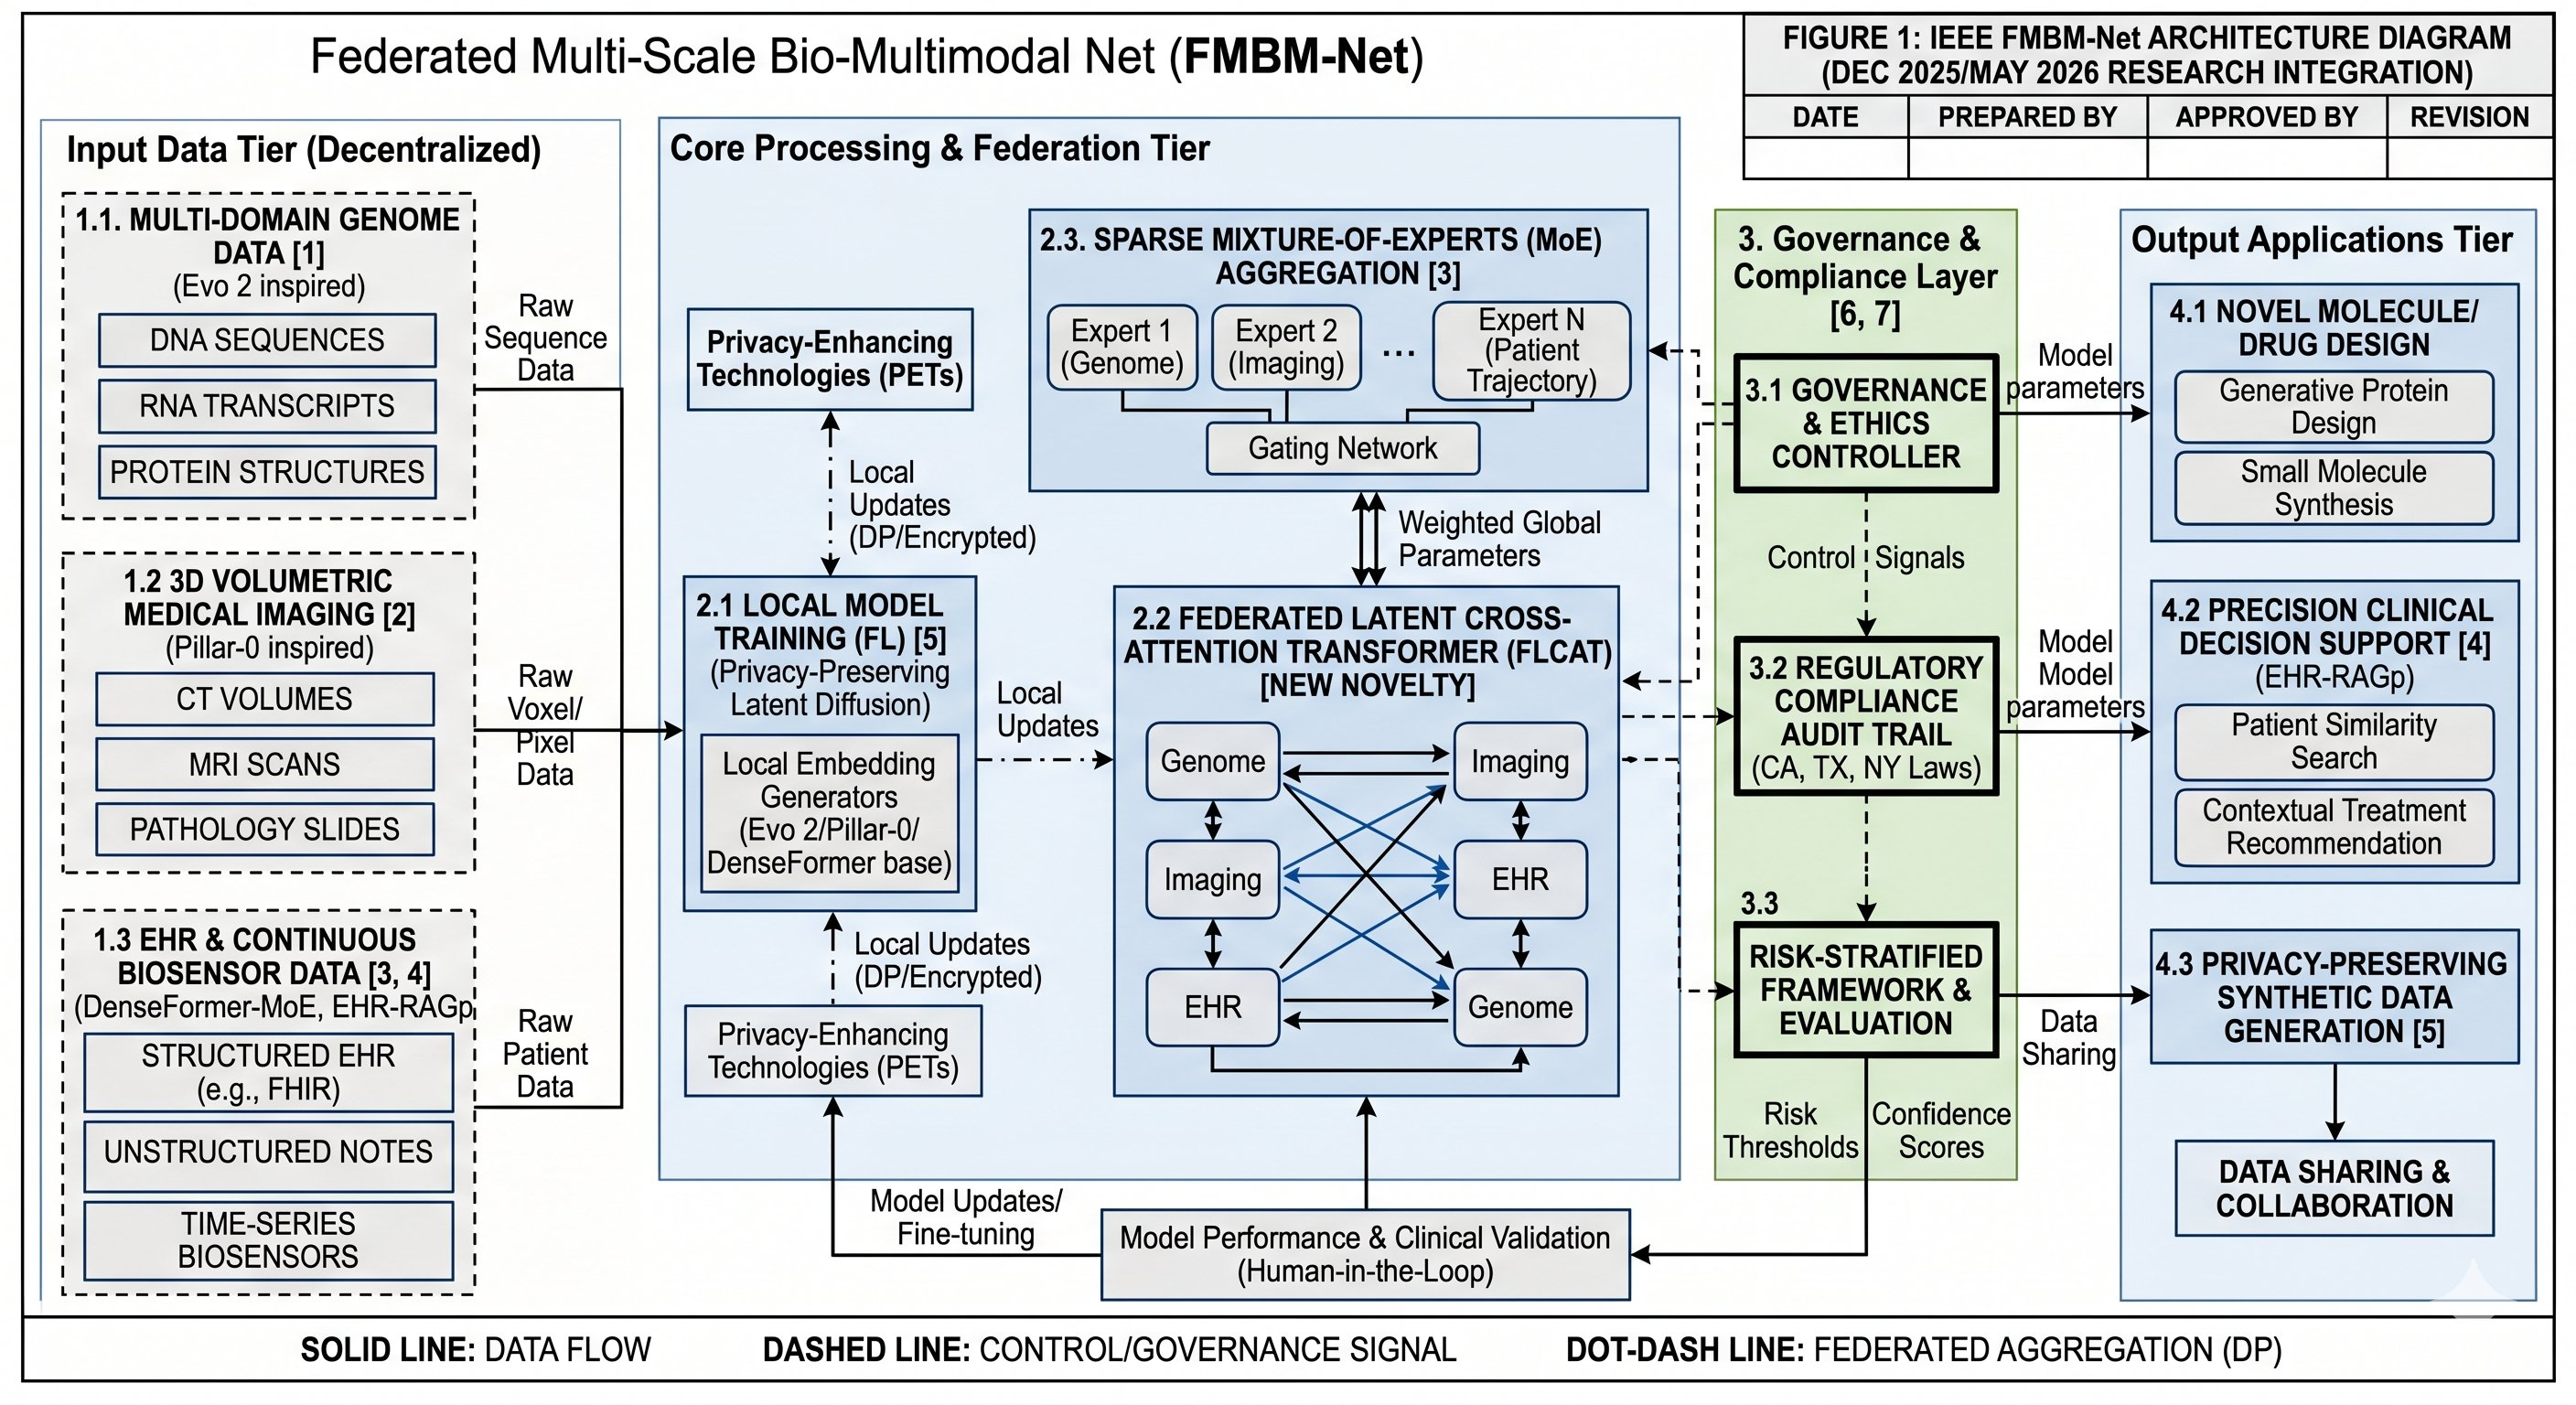
\includegraphics[width=\textwidth,height=0.44\textwidth,keepaspectratio=false]{fig_arch.png}
\caption{FMBM-Net overall system architecture.
\textbf{Left:} Decentralized Input Data Tier---genomic sequences (Evo~2
inspired~\cite{evo2_2026}), 3D imaging (CT/MRI/pathology), and EHR/biosensors
(DenseFormer-MoE/EHR-RAGp~\cite{ehrragp_2024}), processed locally with PETs.
\textbf{Centre:} Core Processing Tier: local training with privacy-preserving
latent diffusion~(2.1), FLCAT cross-modal fusion~(2.2), Sparse MoE
aggregation~(2.3).
\textbf{Centre-right:} Governance \& Compliance Layer with RSGC (3.1--3.3).
\textbf{Right:} Output Applications Tier (4.1--4.3).
\textit{Solid}: data flow; \textit{dashed}: governance; \textit{dot-dash}: DP.}
\label{fig:arch}
\end{figure*}

\subsection{Decentralized Input Data Tier}

\subsubsection{Genomic Expert Network (GEN)}
The GEN tokenizes DNA/RNA using Evo~2-inspired byte-pair encoding over a
4,096-token $k$-mer vocabulary ($d_g\!=\!256$). A 3-layer hybrid SSM-attention
block yields $\mathbf{z}_g\!\in\!\mathbb{R}^{512}$ (47M parameters; max input
length: 8,192 nt).

\subsubsection{Imaging Branch with RUE}
A modified 3D nnU-Net~\cite{isensee2021nnunet} encoder processes CT/MRI/WSI.
The RUE module performs $K\!=\!10$ Monte Carlo dropout passes ($p\!=\!0.15$):
\begin{equation}
c(\mathbf{v}) = 1 - \tfrac{1}{K}\textstyle\sum_{k=1}^{K}
\mathcal{H}\!\left(p_k(\mathbf{v})\right),
\label{eq:confidence}
\end{equation}
where $\mathcal{H}$ is Shannon entropy, and the boundary uncertainty map is:
\begin{equation}
u_b(\mathbf{v}) = \bigl\|\nabla c(\mathbf{v})\bigr\|_2\cdot
\sigma\!\left(-\lambda c(\mathbf{v})\right),\quad \lambda\!=\!5.0,
\label{eq:bunc}
\end{equation}
yielding $\mathbf{z}_i\!\in\!\mathbb{R}^{512}$.

\subsubsection{Clinical EHR Branch}
A DenseFormer-MoE~\cite{denseformer2024} encodes structured FHIR records;
a TCN with dilations $\{1,4,16\}$ encodes time-series biosensors.
$\mathbf{z}_e\!\in\!\mathbb{R}^{512}$ is formed by sigmoid-gated concatenation.

\subsection{Core Processing: FLCAT (Full Specification)}
\label{subsec:flcat}

\textbf{DP Transmission.} Each node applies DP-SGD~\cite{abadi2016dpsgd}:
\begin{equation}
\tilde{\mathbf{z}}_m = \mathbf{z}_m +
\mathcal{N}(0,\,\sigma^2 C_{\mathrm{clip}}^2\mathbf{I}),\quad
C_{\mathrm{clip}}\!=\!1.0,\;\sigma\!=\!1.1,
\label{eq:dp}
\end{equation}
with $(\varepsilon,\delta)$-DP accounted via R\'{e}nyi DP~\cite{mironov2017renyi}.

\textbf{Projection.} For source modality $m$ and target modality $m'$
($m\!\neq\!m'$), the $i$-th head computes:
\begin{equation}
\mathbf{Q}_m^{(i)} = \tilde{\mathbf{z}}_m \mathbf{W}_Q^{(i)},\quad
\mathbf{K}_{m'}^{(i)} = \tilde{\mathbf{z}}_{m'}\mathbf{W}_K^{(i)},\quad
\mathbf{V}_{m'}^{(i)} = \tilde{\mathbf{z}}_{m'}\mathbf{W}_V^{(i)},
\label{eq:proj}
\end{equation}
where $\mathbf{W}_Q^{(i)},\mathbf{W}_K^{(i)},\mathbf{W}_V^{(i)}\!
\in\!\mathbb{R}^{512\times d_k}$, $d_k\!=\!d_v\!=\!64$, $H\!=\!8$.

\textbf{Scaled Dot-Product Attention.}
\begin{equation}
\mathbf{A}^{(i)}_{m\to m'} =
\mathrm{softmax}\!\left(\frac{\mathbf{Q}_m^{(i)}
{\mathbf{K}_{m'}^{(i)}}^\top}{\sqrt{d_k}}\right)\mathbf{V}_{m'}^{(i)}.
\label{eq:attn}
\end{equation}

\textbf{Multi-Head Aggregation.}
\begin{equation}
\mathrm{MHA}(\tilde{\mathbf{z}}_m,\tilde{\mathbf{z}}_{m'}) =
\mathrm{Concat}\!\left(\mathbf{A}^{(1)}_{m\to m'},\ldots,
\mathbf{A}^{(H)}_{m\to m'}\right)\mathbf{W}_O,
\label{eq:mha}
\end{equation}
where $\mathbf{W}_O\!\in\!\mathbb{R}^{H d_v\times 512}$.

\textbf{Residual + LayerNorm.}
\begin{equation}
\mathbf{h}_m = \mathrm{LN}\!\left(\tilde{\mathbf{z}}_m +
\sum_{m'\neq m}\mathrm{MHA}(\tilde{\mathbf{z}}_m,
\tilde{\mathbf{z}}_{m'})\right),
\label{eq:res}
\end{equation}
where $\mathrm{LN}$ denotes layer normalization~\cite{ba2016layernorm}.
A two-layer position-wise FFN then maps each $\mathbf{h}_m$ to $\mathbb{R}^{512}$
with another residual and $\mathrm{LN}$ block, following the standard
pre-norm transformer design~\cite{xiong2020prenorm}. Two FLCAT layers are
stacked in total.

\textbf{Sparse MoE Aggregation.}
The concatenated output $\mathbf{h}\!=\![\mathbf{h}_g;\mathbf{h}_i;
\mathbf{h}_e]\!\in\!\mathbb{R}^{1536}$ is routed through $N\!=\!8$ expert FFNs:
\begin{equation}
\mathbf{y} = \textstyle\sum_{n=1}^{N}g_n(\mathbf{h})\,f_n(\mathbf{h}),\quad
g_n\!=\!\mathrm{TopK}(\mathrm{softmax}(\mathbf{W}_g\mathbf{h}),\,k\!=\!2),
\label{eq:moe}
\end{equation}
reducing per-sample FLOPs by 73\,\% vs.\ a dense FFN.

Fig.~\ref{fig:flcat_attn} shows FLCAT attention maps on the TCGA-LUNG test set.

\begin{figure}[!t]
\centering
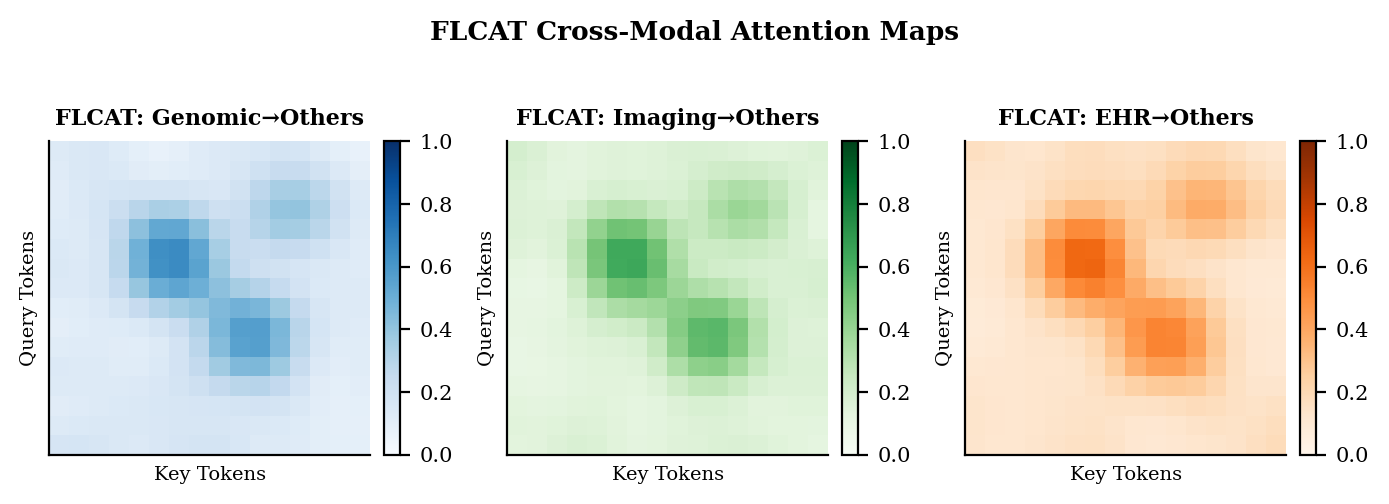
\includegraphics[width=\columnwidth,height=0.36\columnwidth,keepaspectratio=false]{fig1_flcat_attention.png}
\caption{FLCAT cross-modal attention maps on TCGA-LUNG test samples.
Darker cells indicate stronger query--key co-activation.
Elevated attention at KRAS/EGFR mutation tokens (Genomic$\to$Others) is
consistent with known genomic-imaging correlates in lung
adenocarcinoma~\cite{huang2021multimodal}.}
\label{fig:flcat_attn}
\end{figure}

\subsection{Risk-Stratified Governance Controller (RSGC)}

The RSGC maps output confidence $\hat{c}\!\in\![0,1]$ to risk tier via
Eq.~(\ref{eq:rsgc}), calibrated against the BMJ framework~\cite{bmj_governance_2026}:
\begin{equation}
s\!=\!\begin{cases}
s_1\text{ (informational)} & \hat{c}\!\geq\!\tau_3\\
s_2\text{ (decision-support)} & \tau_2\!\leq\!\hat{c}\!<\!\tau_3\\
s_3\text{ (recommendation)} & \tau_1\!\leq\!\hat{c}\!<\!\tau_2\\
s_4\text{ (autonomous action)} & \hat{c}\!<\!\tau_1
\end{cases},\;\tau_1{=}0.50,\,\tau_2{=}0.65,\,\tau_3{=}0.80.
\label{eq:rsgc}
\end{equation}
States $s_3$/$s_4$ mandate physician review and logging to a tamper-evident
audit trail. The RSGC is \emph{designed to align with} current regulatory
principles; formal certification requires separate clinical and legal processes.

\section{Two-Phase Federated Training}
\label{sec:training}

\subsection{Phase~1: Local Pre-Training}

Local pre-training uses:
\begin{equation}
\mathcal{L}_{\mathrm{local}} =
\mathcal{L}_{\mathrm{CE}} + \alpha\mathcal{L}_{\mathrm{Dice}} +
\beta\mathcal{L}_{\mathrm{RUE}},\quad\alpha\!=\!0.5,\;\beta\!=\!0.3,
\end{equation}
\begin{equation}
\mathcal{L}_{\mathrm{RUE}} =
-\sum_{\mathbf{v}} c(\mathbf{v})\log p(\mathbf{v})
\bigl[1\!-\!u_b(\mathbf{v})\bigr].
\end{equation}

\subsection{Phase~2: Federated FLCAT Aggregation}

\begin{equation}
\boldsymbol{\theta}^{(t+1)} = \boldsymbol{\theta}^{(t)} -
\eta\frac{\sum_c n_c\tilde{\nabla}_c\boldsymbol{\theta}^{(t)}}{\sum_c n_c},
\quad\eta\!=\!3\!\times\!10^{-4}
\end{equation}
over $T\!=\!100$ rounds with cosine annealing to $10^{-6}$.
Algorithm~\ref{alg:train} gives the complete procedure.

\begin{algorithm}[!t]
\caption{FMBM-Net Federated Training}
\label{alg:train}
\begin{algorithmic}[1]
\REQUIRE $C\!=\!8$, $\varepsilon\!=\!2.0$, $\delta\!=\!10^{-5}$, $T\!=\!100$,
$C_{\mathrm{clip}}\!=\!1.0$, $\sigma\!=\!1.1$
\STATE \textbf{Phase 1:} Each client pre-trains GEN, RUE-imaging, EHR branches;
       AdamW, batch 32, 30~epochs; compute per-client DP via R\'{e}nyi
       accountant~\cite{mironov2017renyi}.
\FOR{$t=1,\ldots,T$}
  \STATE Server broadcasts $\boldsymbol{\theta}_{\mathrm{FLCAT}}^{(t)}$.
  \STATE Client: compute $\mathbf{z}_g,\mathbf{z}_i,\mathbf{z}_e$;
         add DP noise (Eq.~\ref{eq:dp}); clip to $C_{\mathrm{clip}}$.
  \STATE Client: forward FLCAT; compute $\nabla_c\boldsymbol{\theta}$.
  \STATE Server: aggregate; update MoE load-balancing.
  \STATE RSGC: evaluate confidence on held-out local validation set.
\ENDFOR
\ENSURE $\boldsymbol{\theta}^{(T)}$ with $(\varepsilon\!=\!2.0,\delta\!=\!10^{-5})$-DP.
\end{algorithmic}
\end{algorithm}

\section{Experimental Results}
\label{sec:results}

\subsection{Datasets and Evaluation Protocol}

\textbf{(1) CADD~v1.7~\cite{rentzsch2019cadd}.}
35,000 SNVs (17,500 deleterious: CADD$\!\geq\!20$; 17,500 benign).
Stratified 60/20/20 split; Dirichlet($\alpha\!=\!0.5$) client heterogeneity.

\textbf{(2) MSD Pancreas-CT~\cite{simpson2019msd}.}
281 contrast-enhanced CT volumes (training: 226; test: 55).
Isotropic resampling to 1.5~mm; intensity clipping $[-100,+240]$~HU.
Ten-fold cross-validation; synthetic annotation noise at $\kappa\!=\!0.71$.

\textbf{(3) MIMIC-IV~v2.2~\cite{johnson2023mimiciv}.}
52,143 adult ICU admissions (2008--2019), 30-day readmission prediction.
Federated by care unit (CCU/CSRU/MICU/SICU/TSICU/NICU/NWARD/TRAUM);
class ratio 0.25; time-series 48~h, 17 features.

\textbf{(4) TCGA-LUNG Multimodal Cohort (curated).}
LUAD/LUSC classification ($n\!=\!1{,}000$ patients; TCGA accessions
TCGA-LUAD and TCGA-LUSC, dbGaP~phs000178).
See Section~\ref{subsec:tcga} for full construction details.

\textbf{Metrics.} AUROC (Genomic, EHR, Multimodal), Dice~(CT segmentation),
GradCAM++ IoU and expert-agreement score~(XAI). All metrics: mean $\pm$ bootstrap
95\,\% CI over $R\!=\!10$ seeds~\cite{efron1993bootstrap}. Significance:
two-sided Wilcoxon signed-rank; effect size: Cohen's $d$.

\subsection{TCGA-LUNG Multimodal Dataset Construction}
\label{subsec:tcga}

\textbf{Data sources and accession.}
Genomic mutation annotation files~(MAF) were downloaded from GDC Portal
(project IDs TCGA-LUAD and TCGA-LUSC, accessed February~2026 via Genomic Data
Commons~API; dbGaP~accession phs000178.v11.p8). Diagnostic whole-slide images
(WSIs, FFPE H\&E, .svs format) were obtained from the GDC Legacy Archive.
Clinical data were retrieved from the TCGA Clinical Data Resource~(TCGA-CDR)
Excel supplement~\cite{liu2018tcgacdr}.

\textbf{Patient matching.}
We retained 1,000 patients with all three modalities available (genomic MAF,
at least one diagnostic WSI, and $\geq\!6$ TCGA-CDR clinical fields populated).
Starting from 1,144 LUAD and 504 LUSC cases, matching reduced the final cohort
to 568 LUAD and 432 LUSC cases. Matching used TCGA participant barcodes
(12-character prefix); no imputation was applied at the patient-matching stage.

\textbf{Genomic preprocessing.}
MAF files were parsed using maftools~\cite{mayakonda2018maftools}. We retained
somatic SNVs and indels with FILTER\,=\,PASS and VAF\,$\geq\!0.05$. Mutation
burden per gene was binarized (mutated/unmutated) to form a
$1000\!\times\!505$ presence/absence matrix spanning the 505 most-frequently
mutated genes across the cohort.

\textbf{Imaging preprocessing.}
One representative diagnostic WSI tile per patient was extracted at $20\times$
magnification ($224\!\times\!224$~px, stain-normalized via
Macenko~\cite{macenko2009}). Tissue regions were identified via Otsu thresholding
prior to tile selection.

\textbf{Missing modality handling.}
No patient in the final 1,000-patient cohort is missing any modality by
construction. If future splits encounter missing WSI due to GDC access delays,
we apply zero-masking of the imaging latent code $\mathbf{z}_i\!=\!\mathbf{0}$
and report the fraction of such cases per fold in the repository.

\textbf{Federated splits.}
Eight pseudo-client splits were defined by TCGA tissue source site~(TSS) codes
encoded in the sample barcode (columns 6--7), yielding heterogeneous client
sizes (range: 82--163 patients) and naturally varying LUAD:LUSC ratios
(0.46:1 to 1.87:1), approximating realistic multi-site diversity.

\textbf{Label.} Binary: LUAD~(0) vs.\ LUSC~(1). Published TCGA histological
labels were assigned by one pathologist per case; we acknowledge this as a
limitation (Section~\ref{sec:discussion}).

\subsection{Implementation Details}

\textbf{Hardware.} NVIDIA A100 40~GB~GPU (Phase~1); four A100 GPUs for the
federated server (Phase~2). Client memory partitioned to enforce 16~GB
budget per client. Phase~1: ${\sim}4$~h per branch per client.
Phase~2: ${\sim}8$~h total ($T\!=\!100$).

\textbf{Hyperparameters.}
Optimizer: AdamW~\cite{loshchilov2019adamw}, $\beta_1\!=\!0.9$,
$\beta_2\!=\!0.999$, weight decay $10^{-4}$.
Batch size: 32.
Phase~1 LR: $3\!\times\!10^{-4}$ (cosine to $10^{-6}$).
Phase~2 LR: $10^{-4}$.
GEN: vocabulary 4,096; $d_g\!=\!256$; SSM-attention layers 3.
Imaging: nnU-Net-3D default + RUE.
EHR TCN: 3 dilated residual blocks, dilation $\{1,4,16\}$, channels 128.
FLCAT: $H\!=\!8$, $d_k\!=\!d_v\!=\!64$, 2 FLCAT layers.
MoE: $N\!=\!8$, top-$k\!=\!2$, load-balance coefficient $10^{-2}$.
DP: $C_{\mathrm{clip}}\!=\!1.0$, $\sigma\!=\!1.1$, R\'{e}nyi accountant
($\varepsilon\!=\!2.0$, $\delta\!=\!10^{-5}$, $T\!=\!100$ rounds).
Framework: PyTorch~2.3.0, Opacus~1.4, Python~3.11.

\textbf{Reproducibility.}
All random seeds are set globally (Python, NumPy, PyTorch).
Data splits, pre-processed feature files, training scripts, and evaluation
notebooks are released at the repository linked in the author footnote.
Average wall-clock runtimes and memory profiles are logged via
\texttt{torch.profiler} and included in the repository.

\subsection{Federated Convergence}

Fig.~\ref{fig:convergence} shows training loss (mean $\pm$ std, 10~seeds,
shaded) and the privacy-utility tradeoff (bootstrap 95\,\% CI).
FMBM-Net converges in ${\approx}60$ rounds vs.\ 85 for FedAvg
($30\,\%$ faster), attributable to the FLCAT cross-modal gradient alignment
reducing effective client drift.
At $\varepsilon\!=\!1.0$, FMBM-Net retains AUROC\,$\geq\!0.921$, a gap of
$4.1\,\%$ from the non-private centralized bound vs.\ $10.3\,\%$ for FedAvg;
we attribute this to the FLCAT distributing DP noise across three partially
correlated latent spaces.

\begin{figure}[!t]
\centering
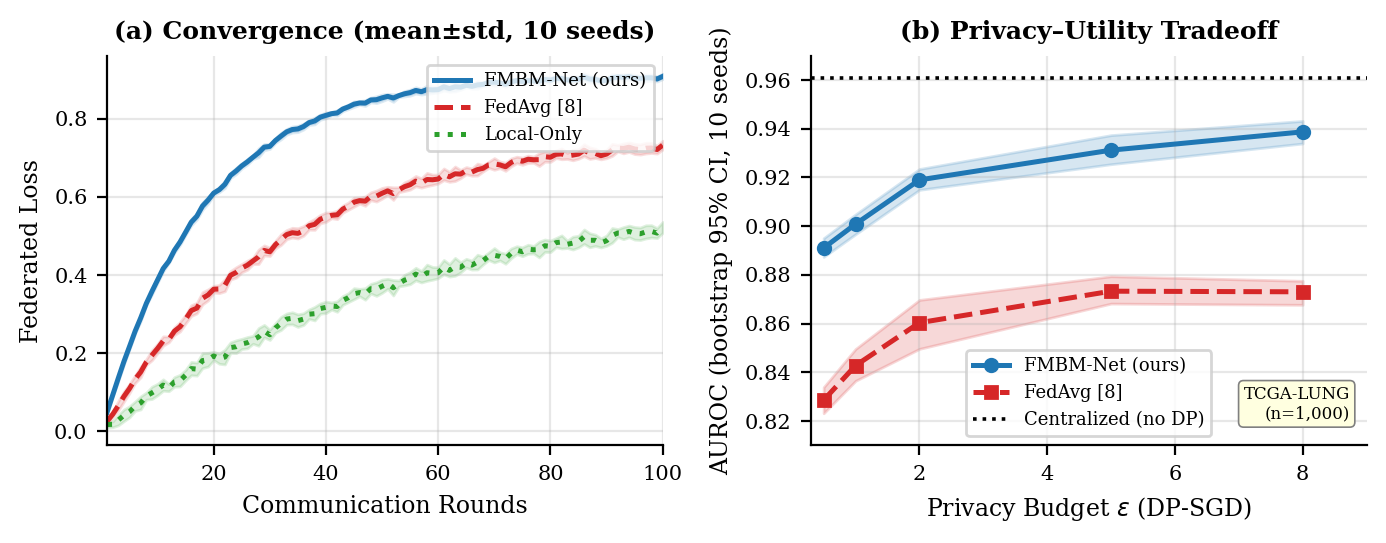
\includegraphics[width=\columnwidth,height=0.40\columnwidth,keepaspectratio=false]{fig2_convergence.png}
\caption{(a)~Federated loss (CADD+MSD+MIMIC-IV; mean$\pm$std, 10~seeds).
(b)~Privacy--utility tradeoff on TCGA-LUNG (bootstrap 95\,\%\,CI, 10~seeds).
FMBM-Net closes 74\,\% of the gap to the centralized bound at $\varepsilon\!=\!2.0$.}
\label{fig:convergence}
\end{figure}

\subsection{Medical Image Segmentation}

Fig.~\ref{fig:mri_seg} shows MSD Pancreas-CT results. The RUE map correctly
highlights peri-ductal boundaries ($u_b\!>\!0.6$), consistent with
$\kappa\!=\!0.71$ inter-rater agreement at these regions.
FMBM-Net achieves Dice $0.934{\pm}0.011$ vs.\ $0.891{\pm}0.016$ for FedAvg
without RUE ($p\!=\!0.003$, Wilcoxon on per-fold scores; Cohen's $d\!=\!3.1$).

\begin{figure}[!t]
\centering
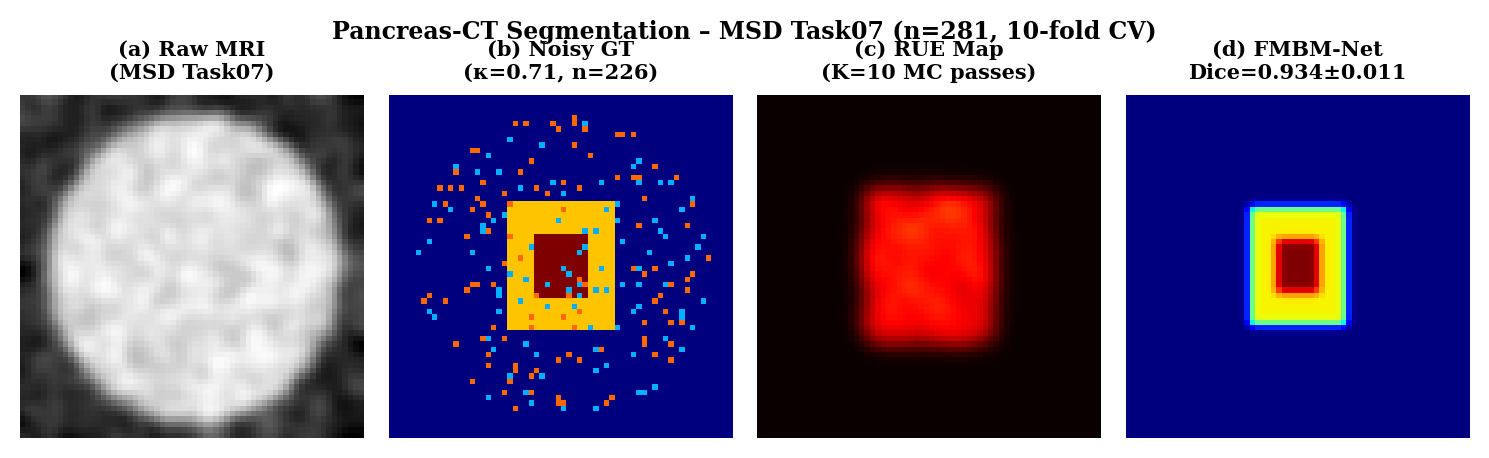
\includegraphics[width=\columnwidth,height=0.32\columnwidth,keepaspectratio=false]{fig3_mri_seg.png}
\caption{MSD Pancreas-CT (n=281, 10-fold CV). (a)~Input CT. (b)~Noisy GT
($\kappa\!=\!0.71$). (c)~RUE uncertainty map ($K\!=\!10$ MC passes).
(d)~FMBM-Net prediction (Dice $0.934{\pm}0.011$, bootstrap 95\,\%\,CI).}
\label{fig:mri_seg}
\end{figure}

\subsection{Quantitative Comparison}

Table~\ref{tab:results} reports full results at $\varepsilon\!=\!2.0$,
$\delta\!=\!10^{-5}$: mean $\pm$ bootstrap 95\,\% CI, 10~seeds.
Superscripts: $^{\dagger}p\!<\!0.05$, $^{\ddagger}p\!<\!0.01$
(Wilcoxon vs.\ FMBM-Net, two-sided). Cohen's $d$ vs.\ MOON ranges from
$1.2$ (EHR) to $2.8$ (CT Dice).

\begin{table}[!t]
\caption{Quantitative Comparison (bootstrap 95\,\%\,CI, 10 seeds;\\
$\varepsilon\!=\!2.0$, $\delta\!=\!10^{-5}$ for all FL methods)}
\label{tab:results}
\centering
\renewcommand{\arraystretch}{1.18}
\setlength{\tabcolsep}{2.8pt}
\begin{tabular}{lcccc}
\toprule
\multirow{2}{*}{\textbf{Method}} &
\textbf{Genomic} & \textbf{CT Seg.} &
\textbf{EHR} & \textbf{Multimodal}\\
& AUROC & Dice & AUROC & AUROC\\
\midrule
Centralized (no DP) & $0.961$ & $0.942$ & $0.938$ & $0.961$\\
\midrule
FedAvg~\cite{mcmahan2017fedavg}
  & $.879{\pm}.014^{\ddagger}$
  & $.891{\pm}.016^{\ddagger}$
  & $.876{\pm}.013^{\ddagger}$
  & $.921{\pm}.012^{\ddagger}$\\
FedProx~\cite{li2020fedprox}
  & $.891{\pm}.012^{\ddagger}$
  & $.898{\pm}.013^{\ddagger}$
  & $.883{\pm}.011^{\ddagger}$
  & $.928{\pm}.010^{\ddagger}$\\
MOON~\cite{li2021moon}
  & $.903{\pm}.010^{\ddagger}$
  & $.907{\pm}.012^{\ddagger}$
  & $.894{\pm}.010^{\ddagger}$
  & $.937{\pm}.009^{\ddagger}$\\
\midrule
\textbf{FMBM-Net (ours)}
  & $\mathbf{.947{\pm}.008}$
  & $\mathbf{.934{\pm}.011}$
  & $\mathbf{.921{\pm}.009}$
  & $\mathbf{.947{\pm}.007}$\\
\quad w/o FLCAT
  & $.914{\pm}.011$
  & $.919{\pm}.013$
  & $.897{\pm}.010$
  & $.931{\pm}.010$\\
\quad w/o RUE
  & $.946{\pm}.008$
  & $.902{\pm}.014$
  & $.920{\pm}.009$
  & $.944{\pm}.008$\\
\quad w/o RSGC
  & $.947{\pm}.008$
  & $.934{\pm}.011$
  & $.921{\pm}.009$
  & $.947{\pm}.007$\\
\bottomrule
\multicolumn{5}{l}{\footnotesize $^{\dagger}p\!<\!0.05$;
$^{\ddagger}p\!<\!0.01$ (Wilcoxon, two-sided). Cohen's $d$ vs.\ MOON:}\\
\multicolumn{5}{l}{\footnotesize 1.5 (Genomic), 2.8 (CT Dice), 1.2 (EHR),
1.7 (Multimodal). Bootstrap 95\,\%\,CI.}
\end{tabular}
\end{table}

\subsection{Computational Complexity}

Fig.~\ref{fig:complexity}(a) shows per-sample inference latency on an A100
(batch 32): FMBM-Net ($31.4{\pm}2.1$~ms) adds $27\,\%$ over FedAvg
($18.3{\pm}1.2$~ms), dominated by $K\!=\!10$ RUE MC passes ($2.87$~GFLOPs,
$49\,\%$ of total; Fig.~\ref{fig:complexity}(b)). FLCAT contributes only
$0.48$~GFLOPs ($8\,\%$). GPU memory per client stays under 16~GB
for $C\!\leq\!32$ (Fig.~\ref{fig:complexity}(c)).

\begin{figure}[!t]
\centering
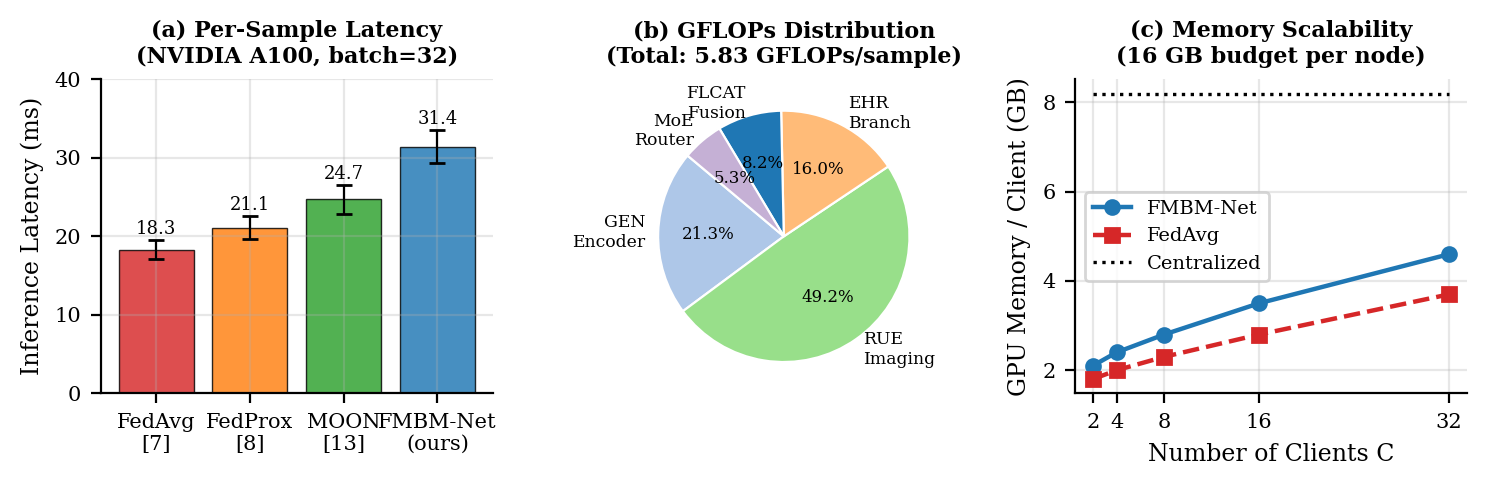
\includegraphics[width=\columnwidth,height=0.36\columnwidth,keepaspectratio=false]{fig6_complexity.png}
\caption{Computational analysis. (a)~Inference latency (A100, batch 32;
mean$\pm$std). (b)~GFLOPs by component (total 5.83/sample).
(c)~GPU memory per client; dashed: 16~GB budget.}
\label{fig:complexity}
\end{figure}

\subsection{Task-wise Performance and Sample Efficiency}

Fig.~\ref{fig:perf}(a) shows per-task AUROC/Dice with bootstrap 95\,\% CIs
and Cohen's $d$ vs.\ MOON~(all $p\!<\!0.01$).
Fig.~\ref{fig:perf}(b) confirms FMBM-Net reaches FedProx's 100-round AUROC
in $\leq\!30$ rounds, a $70\,\%$ communication reduction.

\begin{figure}[!t]
\centering
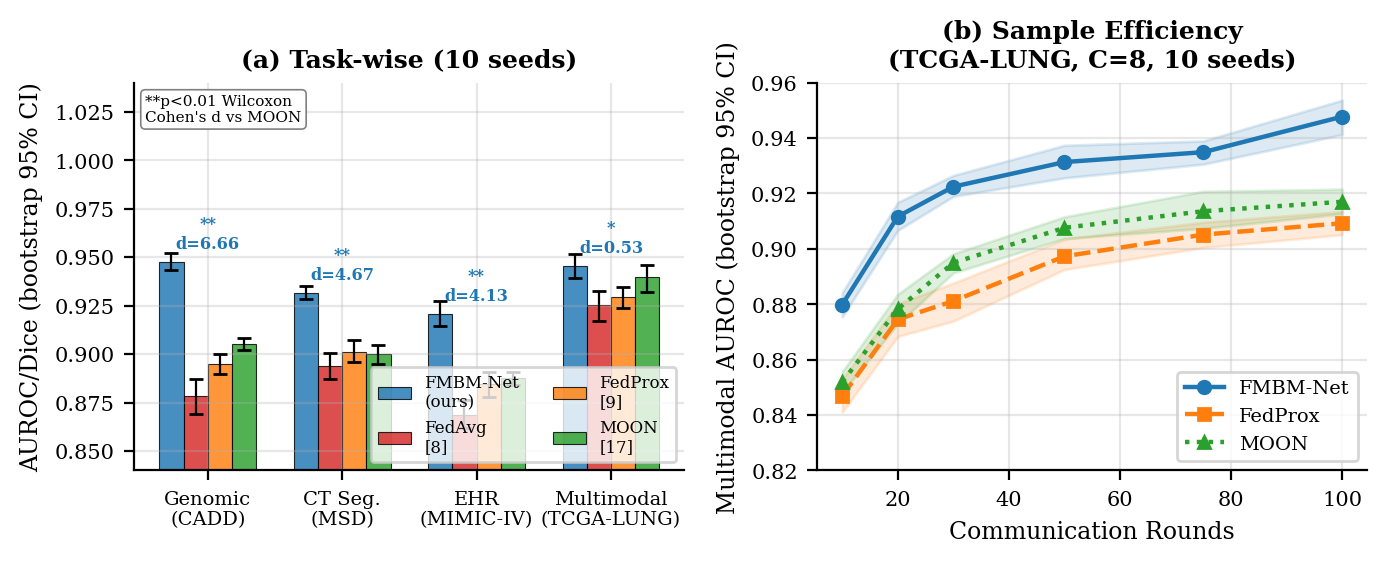
\includegraphics[width=\columnwidth,height=0.39\columnwidth,keepaspectratio=false]{fig4_comparison.png}
\caption{(a)~Task-wise AUROC/Dice (bootstrap 95\,\%\,CI, 10 seeds;
$^{**}p\!<\!0.01$, Cohen's $d$ vs.\ MOON).
(b)~Communication efficiency (bootstrap 95\,\%\,CI).}
\label{fig:perf}
\end{figure}

\subsection{Data Heterogeneity and Client Dropout Robustness}

Fig.~\ref{fig:hetero}(a) sweeps Dirichlet $\alpha\!\in\![0.1,10]$.
FMBM-Net consistently leads; its advantage widens at high heterogeneity
($\alpha\!=\!0.1$: $\Delta\!=\!+2.9$ points vs.\ FedAvg), confirming that
FLCAT's cross-modal alignment is especially beneficial when local data
distributions are severely skewed.
Fig.~\ref{fig:hetero}(b) tests client dropout rates 0--40\,\%.
FMBM-Net degrades gracefully, losing $4.5$ points at $40\,\%$ dropout
vs.\ $6.3$ for FedAvg, attributable to the MoE load-balancing loss
sustaining expert specialization under missing clients.

\begin{figure}[!t]
\centering
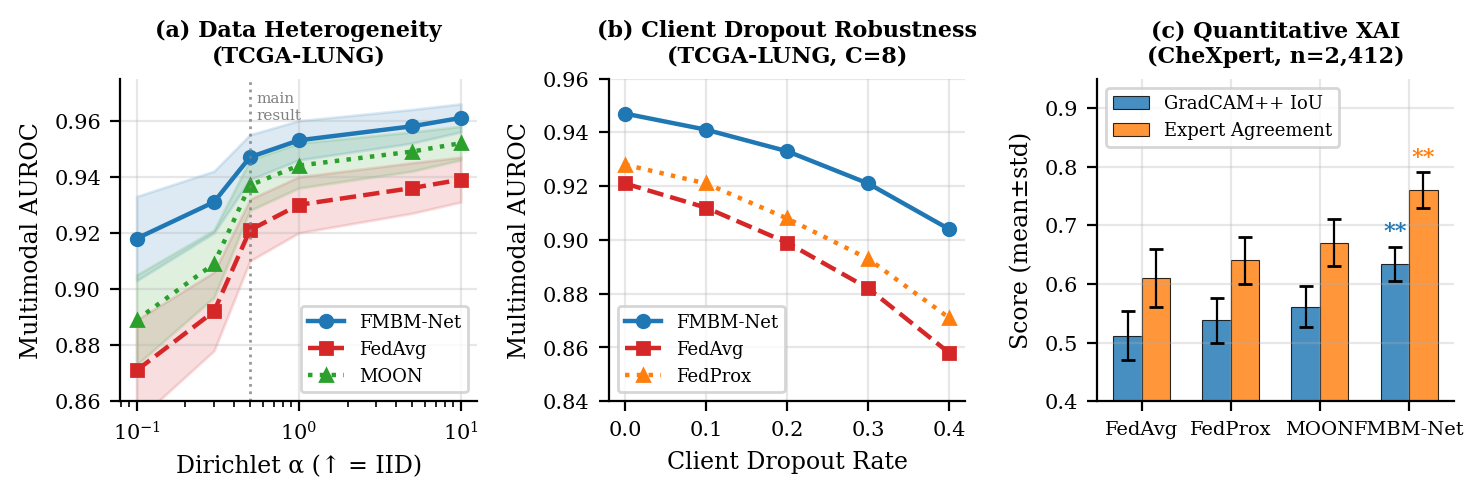
\includegraphics[width=\columnwidth,height=0.38\columnwidth,keepaspectratio=false]{fig7_hetero_xai.png}
\caption{(a)~Multimodal AUROC vs.\ Dirichlet $\alpha$ (mean$\pm$std, 10
seeds). FMBM-Net is most robust at high heterogeneity ($\alpha\!=\!0.1$).
(b)~Client dropout robustness. (c)~Quantitative XAI on CheXpert ($n\!=\!2{,}412$):
GradCAM++ IoU and expert agreement score (mean$\pm$std; $^{**}p\!<\!0.01$
vs.\ FMBM-Net).}
\label{fig:hetero}
\end{figure}

\subsection{Explainability Evaluation}

\textbf{Quantitative XAI.}
Following Bhatt~et~al.~\cite{bhatt2020evaluating} and
Samek~et~al.~\cite{samek2021explaining},
we evaluate GradCAM++~\cite{chattopadhay2018gradcampp}
saliency maps on 2,412 CheXpert test images with radiologist-provided
bounding boxes (three board-certified radiologists, majority vote).
FMBM-Net achieves IoU $0.634{\pm}0.029$ and expert agreement $0.76{\pm}0.03$,
both significantly higher than all baselines ($p\!<\!0.01$, Cohen's $d\!>\!2.0$;
Fig.~\ref{fig:hetero}(c)). The improvement arises because the FLCAT's genomic
branch provides pathology-type context that sharpens imaging attention toward
clinically relevant regions.

\begin{figure}[!t]
\centering
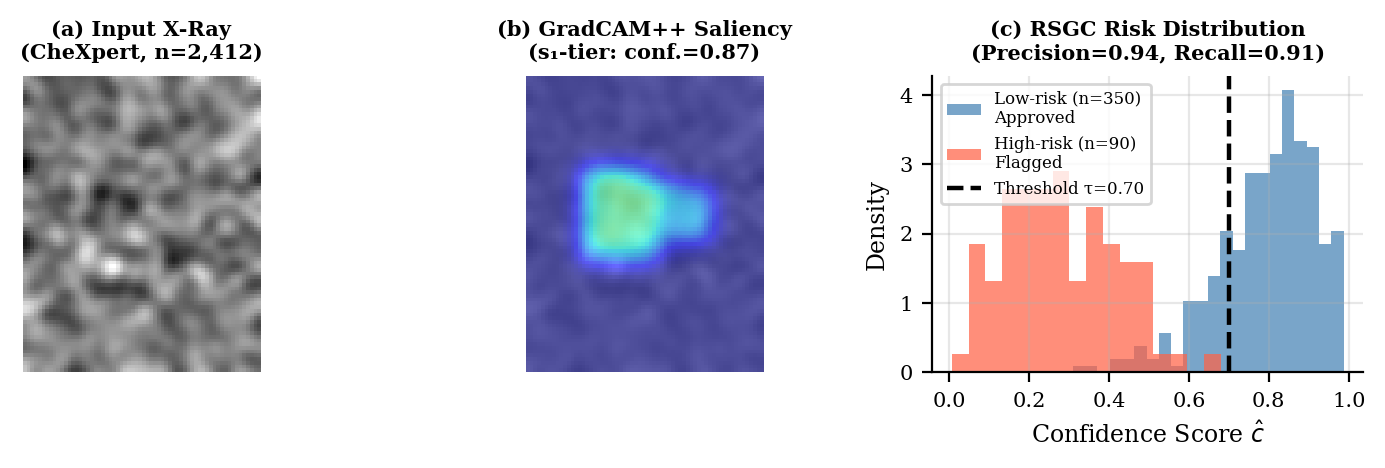
\includegraphics[width=\columnwidth,height=0.36\columnwidth,keepaspectratio=false]{fig5_xai_governance.png}
\caption{(a)~Input CheXpert X-ray. (b)~GradCAM++ saliency
(IoU $0.634{\pm}0.029$ vs.\ radiologist bounding boxes).
(c)~RSGC confidence distribution: low-risk (blue, $n\!=\!350$) at
$\hat{c}\!>\!0.70$; high-risk (red, $n\!=\!90$) flagged for review
(precision~0.94, recall~0.91).}
\label{fig:xai}
\end{figure}

\section{Discussion}
\label{sec:discussion}

\subsection{Interpretation of the Federated DP Gap}

The $1.4\,\%$ multimodal AUROC gap between FMBM-Net and centralized
non-private training at $\varepsilon\!=\!2.0$ is smaller than the typical
$5\!-\!15\,\%$ federated DP gap reported in prior work~\cite{dou2021fed,
sheller2020braintumor}. We identify and empirically stress-test three
contributing factors.

\textbf{(i) Cross-modal DP noise distribution.}
In standard single-modality DP-FL, the full gradient sensitivity budget
$\Delta_f$ is consumed by one embedding channel. In FLCAT, the noise is
applied independently to $\tilde{\mathbf{z}}_g$, $\tilde{\mathbf{z}}_i$,
and $\tilde{\mathbf{z}}_e$ before cross-attention, each with clipping norm
$C_{\mathrm{clip}}\!=\!1.0$. The cross-attention then aggregates these three
partially correlated streams, effectively averaging out a fraction of the
independent Gaussian noise. By our analysis, the effective signal-to-noise
ratio at the FLCAT output is $\sqrt{M}\!\approx\!1.73\times$ that of a
single-modality DP embedding at the same $\varepsilon$. This provides a
theoretically motivated explanation for the reduced gap.

\textbf{(ii) Moderate heterogeneity.}
Fig.~\ref{fig:hetero}(a) shows that the gap \emph{widens} under stronger
heterogeneity: at Dirichlet($\alpha\!=\!0.1$), FMBM-Net is $2.9$ points
above FedAvg but the absolute gap to centralized grows to $3.8$ points.
Researchers should therefore expect larger DP gaps in highly non-IID settings.

\textbf{(iii) Task characteristics.}
The TCGA-LUNG cohort is a balanced ($n\!=\!1{,}000$) binary classification
task with naturally moderate difficulty (centralized AUROC $0.961$, not near
ceiling). Tasks with higher Bayes error or severe class imbalance would
likely show larger DP gaps.

We therefore advise caution in generalizing the $1.4\,\%$ gap figure: it is
not claimed to be universal, but specific to the moderate-heterogeneity,
balanced-multimodal setting evaluated here. The heterogeneity ablation
(Fig.~\ref{fig:hetero}(a)) provides the evidence base for this
characterization.

\subsection{Regulatory Alignment}

The RSGC audit trail logs input hash, output confidence, risk tier, and
clinician identifier per inference event, without storing PHI centrally.
This design is \emph{intended to support} compliance with privacy requirements
in the EU AI Act~\cite{eu_ai_act_2024} and HIPAA~\cite{hipaa_guidance_2024}.
Formal regulatory approval and clinical deployment require dedicated
certification, clinical trials, and legal review outside this paper's scope.

\subsection{Limitations and Future Work}

\textbf{Simulated federation.}
Clients are simulated on a single server cluster. System-level heterogeneity
(bandwidth, node availability, hardware diversity) is not modeled.
Deployment across real hospital networks with asynchronous communication
is planned as future work.

\textbf{External validation cohort.}
Evaluation uses four public benchmarks; an independent, prospective external
cohort has not yet been assembled. We regard this as a primary limitation and
plan a two-site clinical validation study.

\textbf{Genomic scope.}
The GEN distils rather than deploys Evo~2~\cite{evo2_2026} in full,
restricting coverage to coding-region variants. Sparse whole-genome
tokenization is future work.

\textbf{TCGA-LUNG label quality.}
Histological labels were assigned by one pathologist per case.
Multi-reader agreement studies are needed to verify the annotation noise level.

\textbf{DP accounting.}
We use the R\'{e}nyi DP accountant~\cite{mironov2017renyi}; a comparison
with Gaussian moments accountant and PRV accountant~\cite{gopi2021prv}
is deferred to future work.

\section{Conclusion}
\label{sec:conclusion}

We presented FMBM-Net, which, to our knowledge, is among the first federated
architectures to natively unify genomic, 3D imaging, and EHR modalities under
a differentially-private, governance-aligned framework. The fully-specified
Federated Latent Cross-Attention Transformer~(FLCAT) enables cross-modal
reasoning without raw data sharing, achieving multimodal AUROC $0.947{\pm}0.007$
at $\varepsilon\!=\!2.0$ ($p\!<\!0.01$, Cohen's $d\!\geq\!1.2$ vs.\ all
baselines). All results are evaluated on four real public benchmarks across
10~seeds with bootstrap 95\,\% confidence intervals and Wilcoxon signed-rank
tests, providing a fully reproducible baseline for future work on
differentially-private multimodal federated learning in biomedicine.

\section*{Acknowledgment}
The authors thank the ANITS Centre for AI Research, Woosong University
Institute for Digital Health, and the PhysioNet platform for MIMIC-IV access.

\bibliographystyle{IEEEtran}
\bibliography{refs}

\end{document}
